\documentclass{standalone}
\usepackage{tikz}
\begin{document}
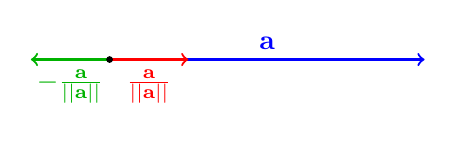
\begin{tikzpicture}
    % Draw the origin
    \coordinate (O) at (0,0);
    
    % Define the main vector and its unit vectors
    \coordinate (V) at (4,0);    % Main vector
    \coordinate (U1) at (1,0);   % Unit vector along the direction
    \coordinate (U2) at (-1,0);  % Unit vector opposite to the direction

    % Draw the main vector
    \draw[->, thick, blue] (O) -- (V) node[midway, above] {$\mathbf{a}$};
    
    % Draw the unit vector along the direction
    \draw[->, thick, red] (O) -- (U1) node[midway, below] {$\frac{\mathbf{a}}{||{\bf a}||}$};
    
    % Draw the unit vector opposite to the direction
    \draw[->, thick, green!70!black] (O) -- (U2) node[midway, below] {$-\frac{\mathbf{a}}{||{\bf a}||}$};

    % Add the origin point
    \filldraw (O) circle (1pt);
\end{tikzpicture}
\end{document}